% Generated by Sphinx.
\def\sphinxdocclass{report}
\documentclass[letterpaper,10pt,english]{sphinxmanual}
\usepackage[utf8]{inputenc}
\DeclareUnicodeCharacter{00A0}{\nobreakspace}
\usepackage{cmap}
\usepackage[T1]{fontenc}
\usepackage{babel}
\usepackage{times}
\usepackage[Bjarne]{fncychap}
\usepackage{longtable}
\usepackage{sphinx}
\usepackage{multirow}


\title{Libellus Documentation}
\date{May 05, 2014}
\release{1.0}
\author{Libellus.no}
\newcommand{\sphinxlogo}{}
\renewcommand{\releasename}{Release}
\makeindex

\makeatletter
\def\PYG@reset{\let\PYG@it=\relax \let\PYG@bf=\relax%
    \let\PYG@ul=\relax \let\PYG@tc=\relax%
    \let\PYG@bc=\relax \let\PYG@ff=\relax}
\def\PYG@tok#1{\csname PYG@tok@#1\endcsname}
\def\PYG@toks#1+{\ifx\relax#1\empty\else%
    \PYG@tok{#1}\expandafter\PYG@toks\fi}
\def\PYG@do#1{\PYG@bc{\PYG@tc{\PYG@ul{%
    \PYG@it{\PYG@bf{\PYG@ff{#1}}}}}}}
\def\PYG#1#2{\PYG@reset\PYG@toks#1+\relax+\PYG@do{#2}}

\expandafter\def\csname PYG@tok@gd\endcsname{\def\PYG@tc##1{\textcolor[rgb]{0.63,0.00,0.00}{##1}}}
\expandafter\def\csname PYG@tok@gu\endcsname{\let\PYG@bf=\textbf\def\PYG@tc##1{\textcolor[rgb]{0.50,0.00,0.50}{##1}}}
\expandafter\def\csname PYG@tok@gt\endcsname{\def\PYG@tc##1{\textcolor[rgb]{0.00,0.27,0.87}{##1}}}
\expandafter\def\csname PYG@tok@gs\endcsname{\let\PYG@bf=\textbf}
\expandafter\def\csname PYG@tok@gr\endcsname{\def\PYG@tc##1{\textcolor[rgb]{1.00,0.00,0.00}{##1}}}
\expandafter\def\csname PYG@tok@cm\endcsname{\let\PYG@it=\textit\def\PYG@tc##1{\textcolor[rgb]{0.25,0.50,0.56}{##1}}}
\expandafter\def\csname PYG@tok@vg\endcsname{\def\PYG@tc##1{\textcolor[rgb]{0.73,0.38,0.84}{##1}}}
\expandafter\def\csname PYG@tok@m\endcsname{\def\PYG@tc##1{\textcolor[rgb]{0.13,0.50,0.31}{##1}}}
\expandafter\def\csname PYG@tok@mh\endcsname{\def\PYG@tc##1{\textcolor[rgb]{0.13,0.50,0.31}{##1}}}
\expandafter\def\csname PYG@tok@cs\endcsname{\def\PYG@tc##1{\textcolor[rgb]{0.25,0.50,0.56}{##1}}\def\PYG@bc##1{\setlength{\fboxsep}{0pt}\colorbox[rgb]{1.00,0.94,0.94}{\strut ##1}}}
\expandafter\def\csname PYG@tok@ge\endcsname{\let\PYG@it=\textit}
\expandafter\def\csname PYG@tok@vc\endcsname{\def\PYG@tc##1{\textcolor[rgb]{0.73,0.38,0.84}{##1}}}
\expandafter\def\csname PYG@tok@il\endcsname{\def\PYG@tc##1{\textcolor[rgb]{0.13,0.50,0.31}{##1}}}
\expandafter\def\csname PYG@tok@go\endcsname{\def\PYG@tc##1{\textcolor[rgb]{0.20,0.20,0.20}{##1}}}
\expandafter\def\csname PYG@tok@cp\endcsname{\def\PYG@tc##1{\textcolor[rgb]{0.00,0.44,0.13}{##1}}}
\expandafter\def\csname PYG@tok@gi\endcsname{\def\PYG@tc##1{\textcolor[rgb]{0.00,0.63,0.00}{##1}}}
\expandafter\def\csname PYG@tok@gh\endcsname{\let\PYG@bf=\textbf\def\PYG@tc##1{\textcolor[rgb]{0.00,0.00,0.50}{##1}}}
\expandafter\def\csname PYG@tok@ni\endcsname{\let\PYG@bf=\textbf\def\PYG@tc##1{\textcolor[rgb]{0.84,0.33,0.22}{##1}}}
\expandafter\def\csname PYG@tok@nl\endcsname{\let\PYG@bf=\textbf\def\PYG@tc##1{\textcolor[rgb]{0.00,0.13,0.44}{##1}}}
\expandafter\def\csname PYG@tok@nn\endcsname{\let\PYG@bf=\textbf\def\PYG@tc##1{\textcolor[rgb]{0.05,0.52,0.71}{##1}}}
\expandafter\def\csname PYG@tok@no\endcsname{\def\PYG@tc##1{\textcolor[rgb]{0.38,0.68,0.84}{##1}}}
\expandafter\def\csname PYG@tok@na\endcsname{\def\PYG@tc##1{\textcolor[rgb]{0.25,0.44,0.63}{##1}}}
\expandafter\def\csname PYG@tok@nb\endcsname{\def\PYG@tc##1{\textcolor[rgb]{0.00,0.44,0.13}{##1}}}
\expandafter\def\csname PYG@tok@nc\endcsname{\let\PYG@bf=\textbf\def\PYG@tc##1{\textcolor[rgb]{0.05,0.52,0.71}{##1}}}
\expandafter\def\csname PYG@tok@nd\endcsname{\let\PYG@bf=\textbf\def\PYG@tc##1{\textcolor[rgb]{0.33,0.33,0.33}{##1}}}
\expandafter\def\csname PYG@tok@ne\endcsname{\def\PYG@tc##1{\textcolor[rgb]{0.00,0.44,0.13}{##1}}}
\expandafter\def\csname PYG@tok@nf\endcsname{\def\PYG@tc##1{\textcolor[rgb]{0.02,0.16,0.49}{##1}}}
\expandafter\def\csname PYG@tok@si\endcsname{\let\PYG@it=\textit\def\PYG@tc##1{\textcolor[rgb]{0.44,0.63,0.82}{##1}}}
\expandafter\def\csname PYG@tok@s2\endcsname{\def\PYG@tc##1{\textcolor[rgb]{0.25,0.44,0.63}{##1}}}
\expandafter\def\csname PYG@tok@vi\endcsname{\def\PYG@tc##1{\textcolor[rgb]{0.73,0.38,0.84}{##1}}}
\expandafter\def\csname PYG@tok@nt\endcsname{\let\PYG@bf=\textbf\def\PYG@tc##1{\textcolor[rgb]{0.02,0.16,0.45}{##1}}}
\expandafter\def\csname PYG@tok@nv\endcsname{\def\PYG@tc##1{\textcolor[rgb]{0.73,0.38,0.84}{##1}}}
\expandafter\def\csname PYG@tok@s1\endcsname{\def\PYG@tc##1{\textcolor[rgb]{0.25,0.44,0.63}{##1}}}
\expandafter\def\csname PYG@tok@gp\endcsname{\let\PYG@bf=\textbf\def\PYG@tc##1{\textcolor[rgb]{0.78,0.36,0.04}{##1}}}
\expandafter\def\csname PYG@tok@sh\endcsname{\def\PYG@tc##1{\textcolor[rgb]{0.25,0.44,0.63}{##1}}}
\expandafter\def\csname PYG@tok@ow\endcsname{\let\PYG@bf=\textbf\def\PYG@tc##1{\textcolor[rgb]{0.00,0.44,0.13}{##1}}}
\expandafter\def\csname PYG@tok@sx\endcsname{\def\PYG@tc##1{\textcolor[rgb]{0.78,0.36,0.04}{##1}}}
\expandafter\def\csname PYG@tok@bp\endcsname{\def\PYG@tc##1{\textcolor[rgb]{0.00,0.44,0.13}{##1}}}
\expandafter\def\csname PYG@tok@c1\endcsname{\let\PYG@it=\textit\def\PYG@tc##1{\textcolor[rgb]{0.25,0.50,0.56}{##1}}}
\expandafter\def\csname PYG@tok@kc\endcsname{\let\PYG@bf=\textbf\def\PYG@tc##1{\textcolor[rgb]{0.00,0.44,0.13}{##1}}}
\expandafter\def\csname PYG@tok@c\endcsname{\let\PYG@it=\textit\def\PYG@tc##1{\textcolor[rgb]{0.25,0.50,0.56}{##1}}}
\expandafter\def\csname PYG@tok@mf\endcsname{\def\PYG@tc##1{\textcolor[rgb]{0.13,0.50,0.31}{##1}}}
\expandafter\def\csname PYG@tok@err\endcsname{\def\PYG@bc##1{\setlength{\fboxsep}{0pt}\fcolorbox[rgb]{1.00,0.00,0.00}{1,1,1}{\strut ##1}}}
\expandafter\def\csname PYG@tok@kd\endcsname{\let\PYG@bf=\textbf\def\PYG@tc##1{\textcolor[rgb]{0.00,0.44,0.13}{##1}}}
\expandafter\def\csname PYG@tok@ss\endcsname{\def\PYG@tc##1{\textcolor[rgb]{0.32,0.47,0.09}{##1}}}
\expandafter\def\csname PYG@tok@sr\endcsname{\def\PYG@tc##1{\textcolor[rgb]{0.14,0.33,0.53}{##1}}}
\expandafter\def\csname PYG@tok@mo\endcsname{\def\PYG@tc##1{\textcolor[rgb]{0.13,0.50,0.31}{##1}}}
\expandafter\def\csname PYG@tok@mi\endcsname{\def\PYG@tc##1{\textcolor[rgb]{0.13,0.50,0.31}{##1}}}
\expandafter\def\csname PYG@tok@kn\endcsname{\let\PYG@bf=\textbf\def\PYG@tc##1{\textcolor[rgb]{0.00,0.44,0.13}{##1}}}
\expandafter\def\csname PYG@tok@o\endcsname{\def\PYG@tc##1{\textcolor[rgb]{0.40,0.40,0.40}{##1}}}
\expandafter\def\csname PYG@tok@kr\endcsname{\let\PYG@bf=\textbf\def\PYG@tc##1{\textcolor[rgb]{0.00,0.44,0.13}{##1}}}
\expandafter\def\csname PYG@tok@s\endcsname{\def\PYG@tc##1{\textcolor[rgb]{0.25,0.44,0.63}{##1}}}
\expandafter\def\csname PYG@tok@kp\endcsname{\def\PYG@tc##1{\textcolor[rgb]{0.00,0.44,0.13}{##1}}}
\expandafter\def\csname PYG@tok@w\endcsname{\def\PYG@tc##1{\textcolor[rgb]{0.73,0.73,0.73}{##1}}}
\expandafter\def\csname PYG@tok@kt\endcsname{\def\PYG@tc##1{\textcolor[rgb]{0.56,0.13,0.00}{##1}}}
\expandafter\def\csname PYG@tok@sc\endcsname{\def\PYG@tc##1{\textcolor[rgb]{0.25,0.44,0.63}{##1}}}
\expandafter\def\csname PYG@tok@sb\endcsname{\def\PYG@tc##1{\textcolor[rgb]{0.25,0.44,0.63}{##1}}}
\expandafter\def\csname PYG@tok@k\endcsname{\let\PYG@bf=\textbf\def\PYG@tc##1{\textcolor[rgb]{0.00,0.44,0.13}{##1}}}
\expandafter\def\csname PYG@tok@se\endcsname{\let\PYG@bf=\textbf\def\PYG@tc##1{\textcolor[rgb]{0.25,0.44,0.63}{##1}}}
\expandafter\def\csname PYG@tok@sd\endcsname{\let\PYG@it=\textit\def\PYG@tc##1{\textcolor[rgb]{0.25,0.44,0.63}{##1}}}

\def\PYGZbs{\char`\\}
\def\PYGZus{\char`\_}
\def\PYGZob{\char`\{}
\def\PYGZcb{\char`\}}
\def\PYGZca{\char`\^}
\def\PYGZam{\char`\&}
\def\PYGZlt{\char`\<}
\def\PYGZgt{\char`\>}
\def\PYGZsh{\char`\#}
\def\PYGZpc{\char`\%}
\def\PYGZdl{\char`\$}
\def\PYGZhy{\char`\-}
\def\PYGZsq{\char`\'}
\def\PYGZdq{\char`\"}
\def\PYGZti{\char`\~}
% for compatibility with earlier versions
\def\PYGZat{@}
\def\PYGZlb{[}
\def\PYGZrb{]}
\makeatother

\begin{document}

\maketitle
\tableofcontents
\phantomsection\label{index::doc}



\chapter{1.   Introduction}
\label{Introduction:introduction}\label{Introduction::doc}\label{Introduction:libellus-1-0-documentation}
Libellus is an open source and ultra portable journal tool for crisis management. It runs in all modern web browsers, ready to use out of the box.


\chapter{User manual}
\label{User manual::doc}\label{User manual:user-manual}

\section{Start Libellus}
\label{User manual:start-libellus}
To start Libellus, find the file on the USB-drive with the name matching your operating system.
If you are running Microsoft Windows 7 or 8, the name of the file will be \emph{windows.bat}.
\begin{figure}[htbp]
\centering
\capstart

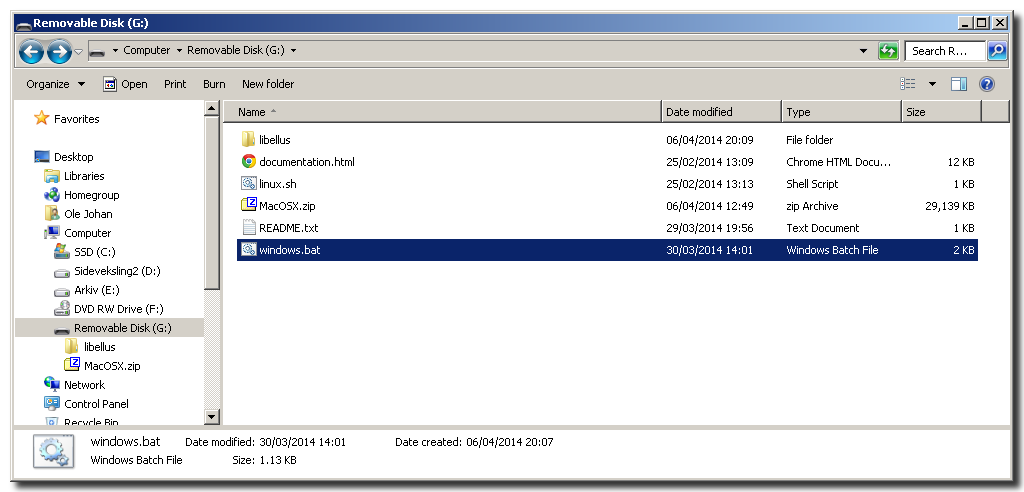
\includegraphics{folder.png}
\caption{This window shows the folder structure on a windows-machine.}\end{figure}

This file is a startup script that will perform some processes in the background to get Libellus up and running. All the actions will be run from a console window.
\begin{figure}[htbp]
\centering
\capstart

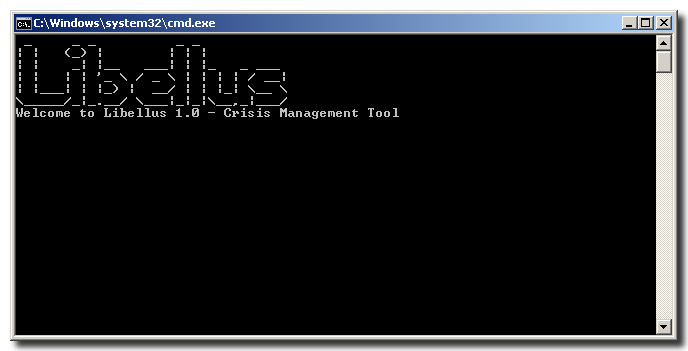
\includegraphics{console.png}
\caption{This is the typical console-window. Here shown on a computer running Microsoft Windows.}\end{figure}

Normally all user accounts can run this file, but if the script senses that it needs elevation, you will be prompted with a message telling you how to do this.

Libellus will be needing access to the network for communication with other running instances of the software. To enable this, click allow access in the two dialog boxes asking for permissions.
\begin{figure}[htbp]
\centering

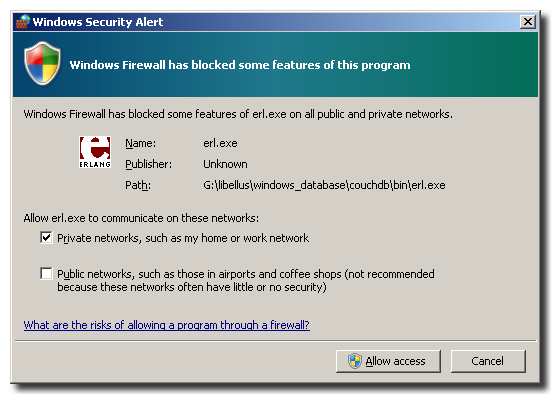
\includegraphics{fw_erl.png}
\end{figure}
\begin{figure}[htbp]
\centering

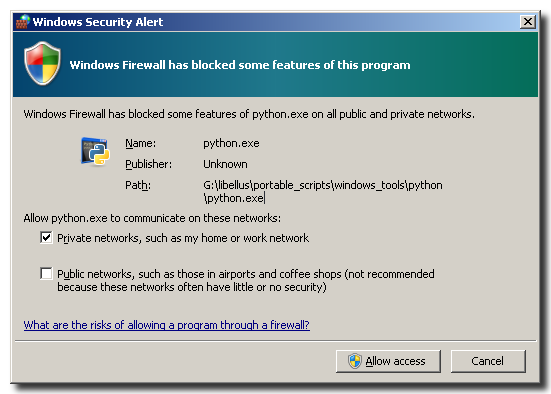
\includegraphics{fw_python.png}
\end{figure}

After some seconds, your default browser will open and be directed at the localhost address (\href{https://127.0.0.1:6984/libellus/index.html}{https://127.0.0.1:6984/libellus/index.html})
All communication in Libellus is transferred encrypted using the TLS technology. To enable this to run on a local computer, Libellus uses a self-signed certificate. This will make your browser display a warning message like the one below. Click on \emph{Proceed anyway} to continue.
\begin{figure}[htbp]
\centering

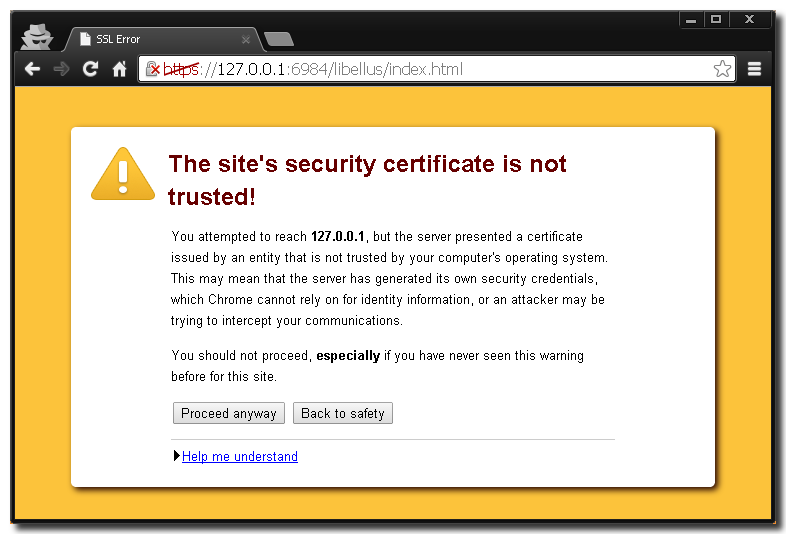
\includegraphics{ssl.png}
\end{figure}


\section{Login}
\label{User manual:login}
After the startup process, the following screen is the first you will meet.
\begin{figure}[htbp]
\centering

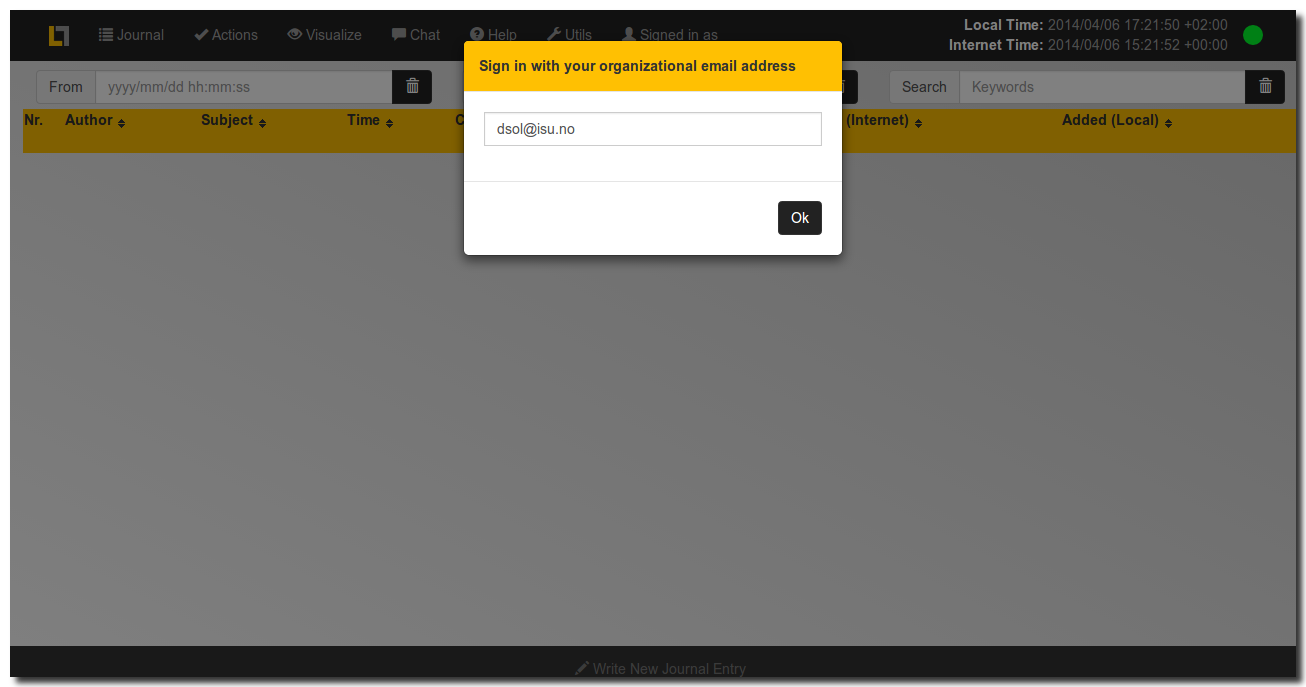
\includegraphics{startscreen.png}
\end{figure}

The only thing you need to enter before you can use the program is a username. There is no users registered beforehand, which makes this the registration. The username can be whatever you want it to be, but we suggest to use something that identifies you, as well to be unique. Your first name will not be a good idea, because there are others with the same first name. We recommend your organizational email address, because it’s globally unique and will usually identify you by the screen name. If you need to change the username, this can be done by clicking on the \emph{Signed in as \textless{}username\textgreater{}} on the menu.


\section{Clock}
\label{User manual:clock}
In the upper right corner, you will see two datetimes. Local Time is the time taken from your computer, which is presented in the local timezone the computer is set to. Internet Time is a time taken from an external source on the Internet. This will always be presented in UTC plus 0 hours. If the Local Time and Internet Time is more or less in sync, the circle on the right side will be green. If both clocks are more than 3 seconds apart, the circle will be orange. If Libellus doesn’t have access to the Internet, the green circle will be red. You can also hold your mouse over the circle and it will show you the offset between both times.
\begin{figure}[htbp]
\centering

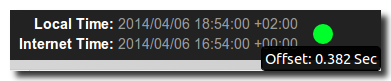
\includegraphics{clock.png}
\end{figure}

If the clocks are not in sync, we recommend that you change your computer time manually, or that you update it automatically. You can’t do this from Libellus, but most operating systems support it. We suggest that all clients on the network have the same local time.

Every entry will be stored with local time, and if Libellus has access to Internet time, it will also store this. Even if you start to log without Internet time, but get access later, Libellus will calculate the offset and update every entry and add Internet time. As another method to ensure integrity, Libellus will log every time the client change the computer time.


\section{The Journal View}
\label{User manual:the-journal-view}
The default screen is the journal view, which is probably where you will spend the most time.
Right under the main menu, you can see some filtering options, which we will cover later, when we got some data to apply filters to.
\begin{figure}[htbp]
\centering

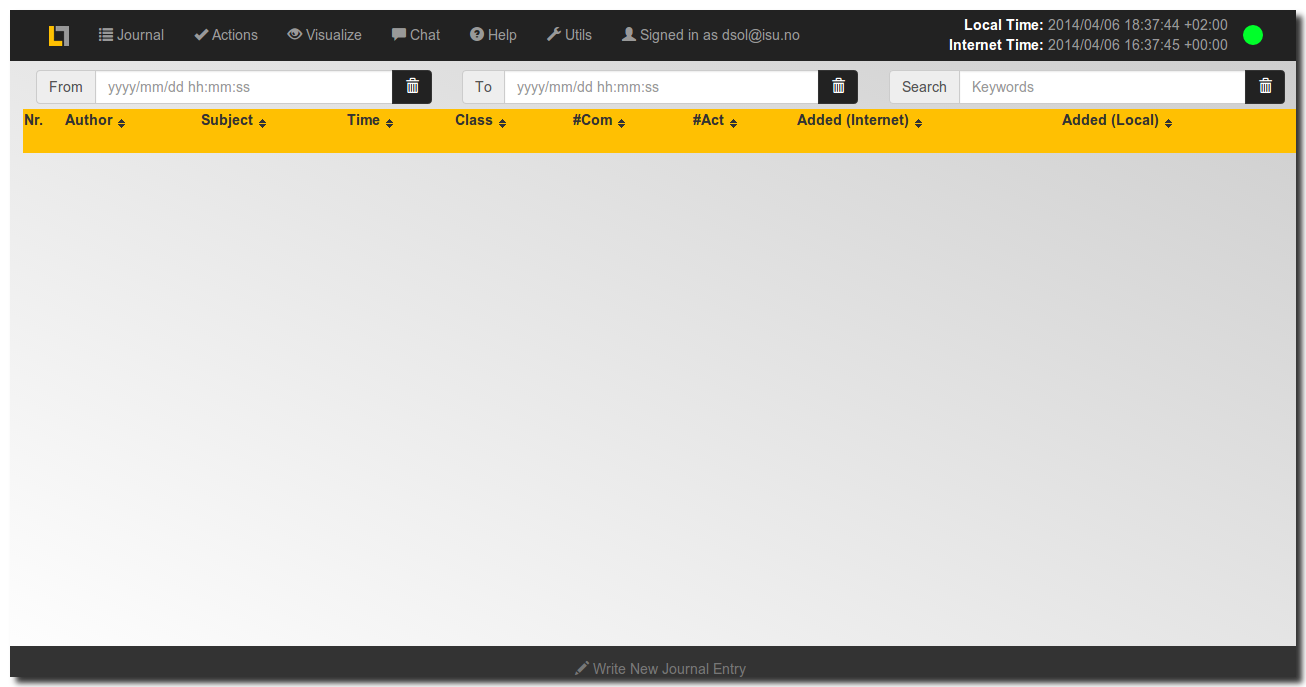
\includegraphics{journal8.png}
\end{figure}

Under the filtering options, you see some headers for the table. Here is the explanations for all the columns
\begin{itemize}
\item {} 
\textbf{Nr.} - This is a running number to have something to refer to.

\item {} 
\textbf{Author} - This is the user that made the journal entry

\item {} 
\textbf{Subject} - The subject of the entry.

\item {} 
\textbf{Time} - This is the happening time, when the event took place

\item {} 
\textbf{Class} - This is the classification of the entry. Hold your pointer over the text to show the full content.

\item {} 
\textbf{\#Com} - This is number of comments to the journal entry

\item {} 
\textbf{\#Act} - This is the number of actions to the journal entry

\item {} 
\textbf{Added (Internet)} - This is the time taken from an external source on the Internet, when the entry was stored into the Libellus client. This may be displaying N/A if the client didn’t have access to the Internet when the entry was stored.

\item {} 
\textbf{Added (Local)} - This is the time taken from the clients computer when the entry was stored in the the database

\end{itemize}

The last thing you may have noticed is the footer at the bottom with the caption Write New Journal Entry, which will be covered next.


\section{Write New Journal Entry}
\label{User manual:write-new-journal-entry}
When you have clicked on the \emph{Write New Journal Entry} bar, a form will appear. The subject should explain in short what the entry is about and content should contain the full story of the event. Keywords is a free text input field, where you can write words to associate the entry with. This is a feature to make it easier to search for entries later. \emph{Happening time} should be in the past, when the event you are writing about took place. This should not be confused with \emph{Added (Internet)} or \emph{Added (Local)}, which is when the journal entry was added. The drop down menu with predefined classification values should describe who can know about the information you are writing about. Libellus does not handle classification different, but the organization that use Libellus might.
\begin{figure}[htbp]
\centering

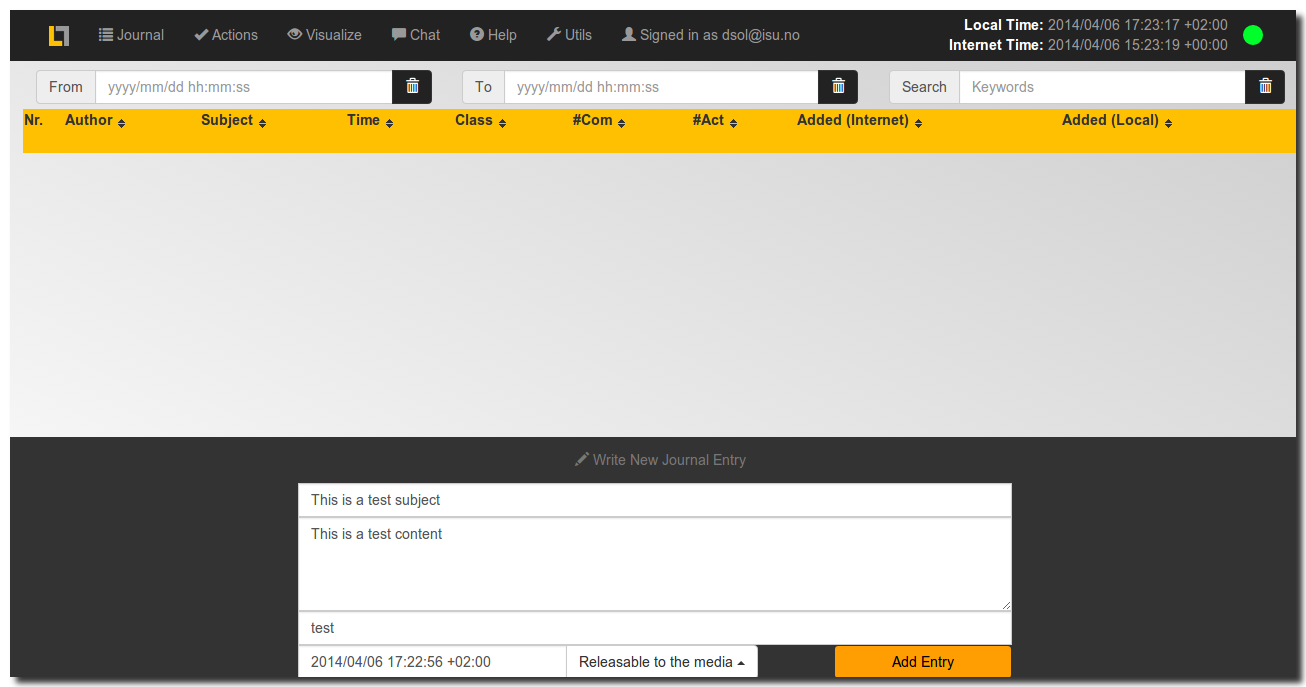
\includegraphics{journal1.png}
\end{figure}

When you have filled in the values and clicked on \emph{Add Entry}, you can close the form by clicking on it again. You can now see that the entry is displayed in the journal, and you can expand it by simply clicking on it. Now your screen should look something like the following.
\begin{figure}[htbp]
\centering

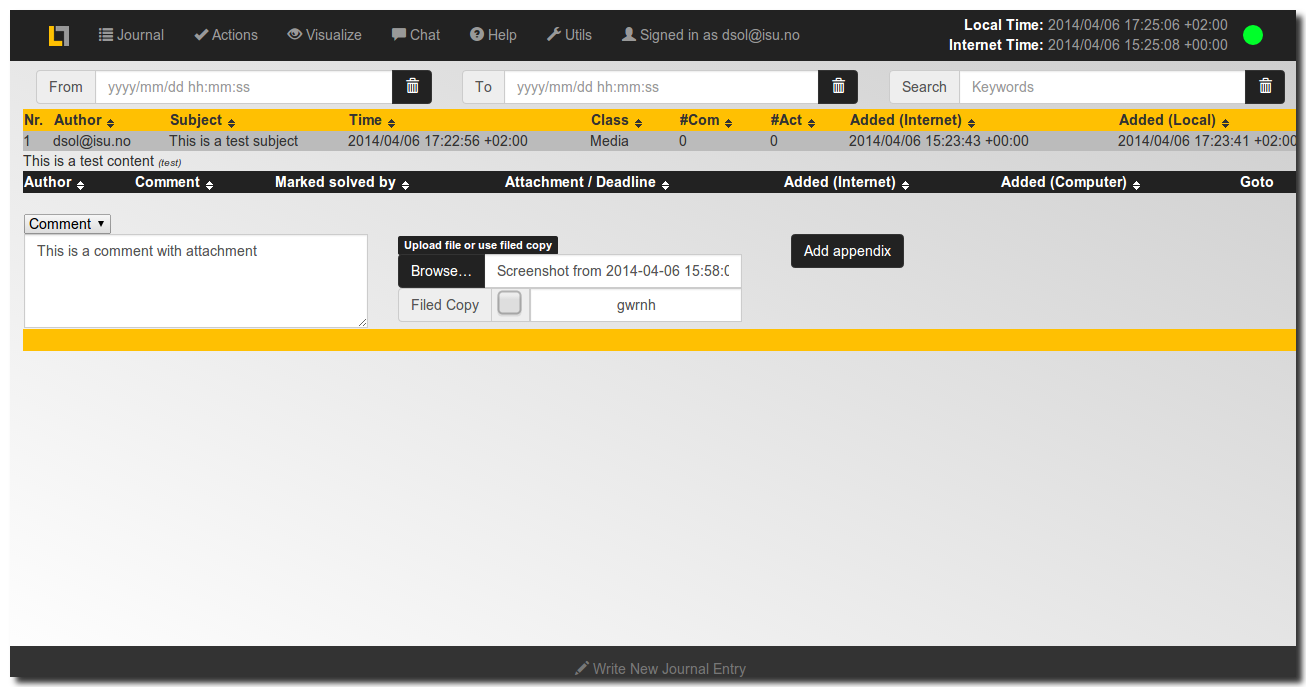
\includegraphics{journal2.png}
\end{figure}

Notice that you can find the content and keywords under the row with metadata.


\section{Appendices}
\label{User manual:appendices}
As you can see in the previous image, there is a form inside the journal table. This is where you can add appendices, i.e. comments and actions. The first drop down menu you see is where
you choose whether to create a comment or action. The difference of these alternatives, is that a comment is to add information to the journal entry and actions is anything that needs to be done in relations to the journal entry.


\subsection{Comments}
\label{User manual:comments}
When creating a comment, you have two choices of the type of attachment. The first is to upload a digital file. Just hit the browse button and a file manager will appear, where you can find your file, but be careful to not upload large files. This is because the file may be replicated amongst many clients and take up much bandwidth. The default max file size is set to 10 megabytes. The second alternative is filed copy.
\begin{figure}[htbp]
\centering

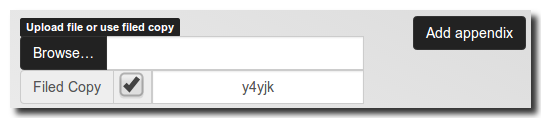
\includegraphics{filed_copy.png}
\end{figure}

Let's say you have a physical paper, hard drive, CD or basically something that you can't upload, or is too big to be uploaded, but you want the journal to keep a record of. Filed copy makes you do this, by a random generated reference string. Check the filed copy checkbox and write the string on the physical object, or maybe use a post-it note on it, before you hit the submit button.


\subsection{Actions}
\label{User manual:actions}
To add an action instead of a comment, just change the value on the drop down box. Now you will see some other input fields. Here you can write a deadline to when the action needs to be complete. When clicking in the field, it will get a default value, which is the current date and time, but should be set to a time in the future. The second new input field is who is responsible for the task. This could be his screen name on Libellus or his real name, but it’s up to the organization to choose what to use.
\begin{figure}[htbp]
\centering

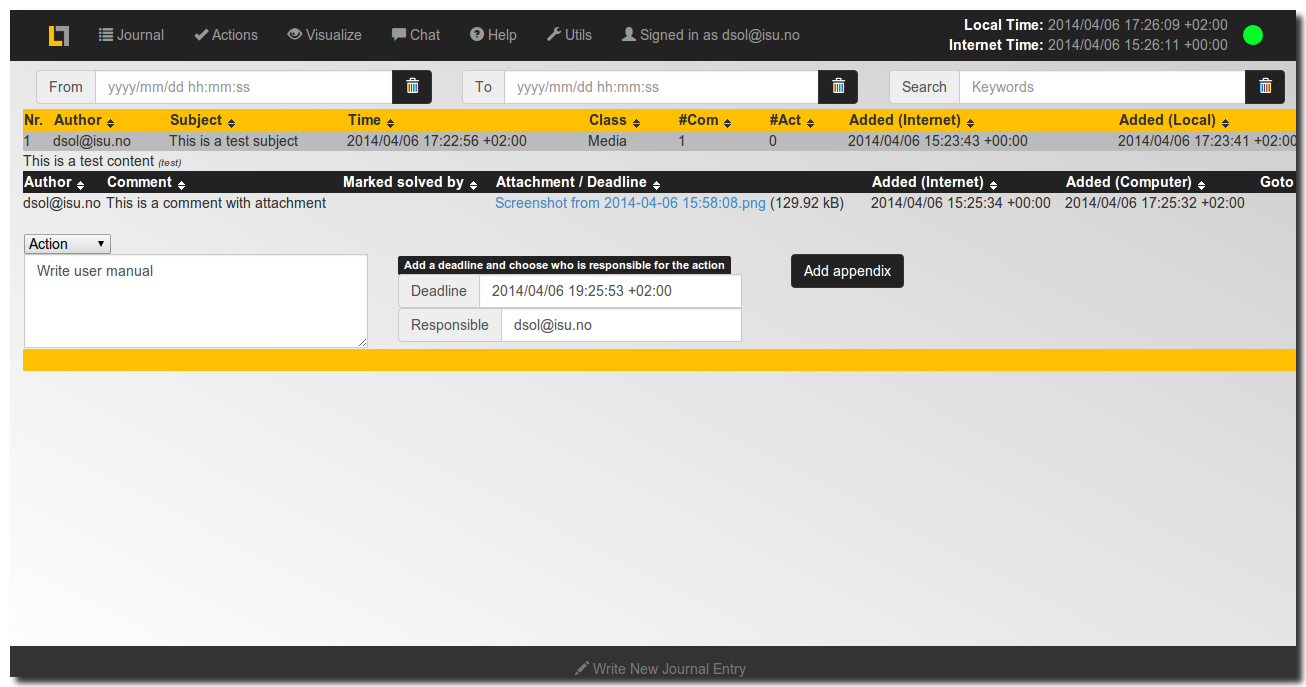
\includegraphics{journal3.png}
\end{figure}

When the action is added, you will see that the entry like in the image below. The row is highlighted in blue, because the deadline is over an hour due in the future. The color will change to orange when the deadline is less than an hour and turn red when the time limit is in the past. The row will be green when the action is solved, and get a strike through when rejected, which we will get to later.
\begin{figure}[htbp]
\centering

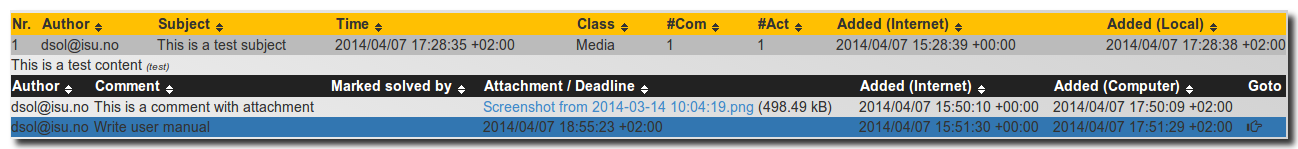
\includegraphics{actions.png}
\end{figure}

There is another feature that comments doesn't have, which is a goto link on the right, depicted with a pointing finger. When clicking on it, you will be directed to the \emph{Actions View} and the target action entry will be expanded.


\section{Sorting}
\label{User manual:sorting}
You can sort every table by clicking on the headers. Click once for descending and twice for ascending sorting. You can also sort by multiple values by holding down the shift key while clicking.


\section{The Actions View}
\label{User manual:the-actions-view}
You can get to the action page by either clicking on Actions in the main menu, or click goto on the inline action entry. The first thing you can notice, is the button on the right, which has changed color to orange in the time between. This button will like the row on the journal page, change color according to the time left for the deadline. The caption on the button now displays \emph{Unsolved}, naturally because no one has solved it yet. The metadata is just like before, but with one exception, that is \emph{Marked solved by}, which is who updated the status of the entry.
\begin{figure}[htbp]
\centering

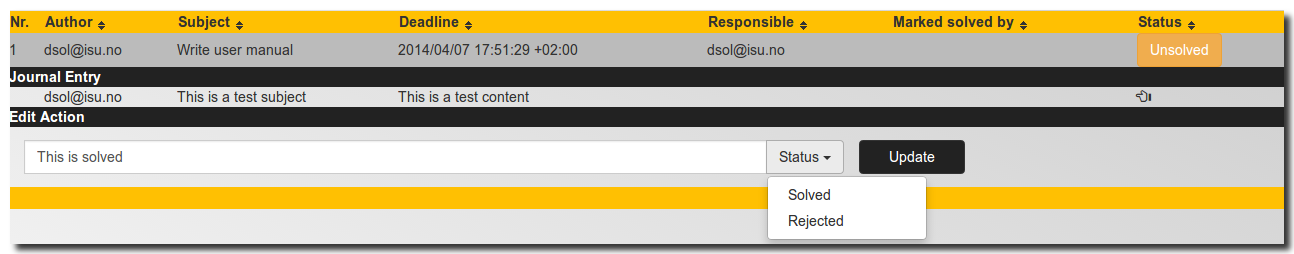
\includegraphics{actions6.png}
\end{figure}

We can also see the complete journal entry that the action are referring to. This is because you can read it and instantly know which journal entry the action are referring to. You also have a goto button here on the right side, which will take you back to the target entry in the journal view.

If an action is solved, just write a comment and select \emph{Solved} in the drop down menu. Now this is what you will see. The status button now displays \emph{Solved} with a green background. The comment and who marked it also are shown.
\begin{figure}[htbp]
\centering

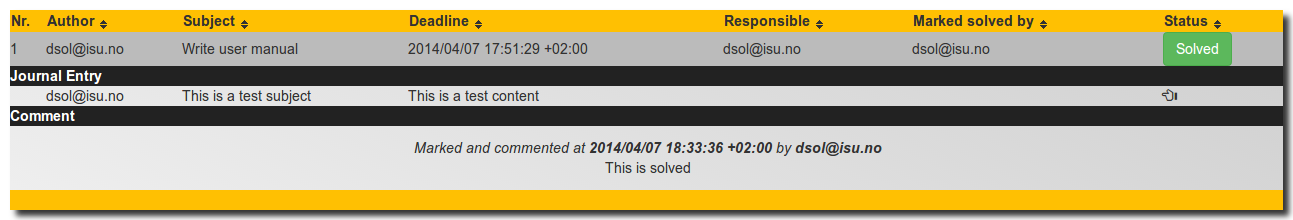
\includegraphics{actions5.png}
\end{figure}

The other alternative to an action is to reject it. This can be useful if the action is not possible to complete or that the deadline is too strict. The image below illustrates how this looks like.
\begin{figure}[htbp]
\centering

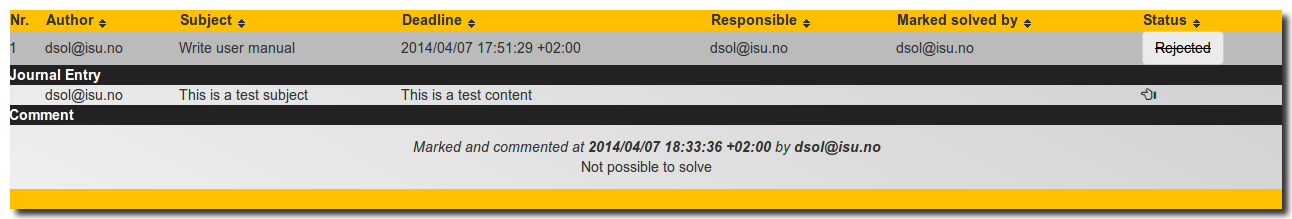
\includegraphics{actions7.png}
\end{figure}

Note that once an action is marked it can not be edited later.


\section{The Visualize View}
\label{User manual:the-visualize-view}
The visualize view shows the journal information on a different perspective. In the example below, you can see a journal entry and an action. Actions will follow the same coloring as they do on the other views, and stretch in length according to the time frame given by the deadline. Use the buttons to navigate in the timeline, or hold and move your mouse in the direction you want to expand the timeline to left or right. You can also zoom in and out with the scroll wheel on your mouse. As you can see, there is a red vertical line in the timeline. This is to mark the current time, which you can always move instantly to by clicking on the button with the caption \emph{Move to current time}.
\begin{figure}[htbp]
\centering

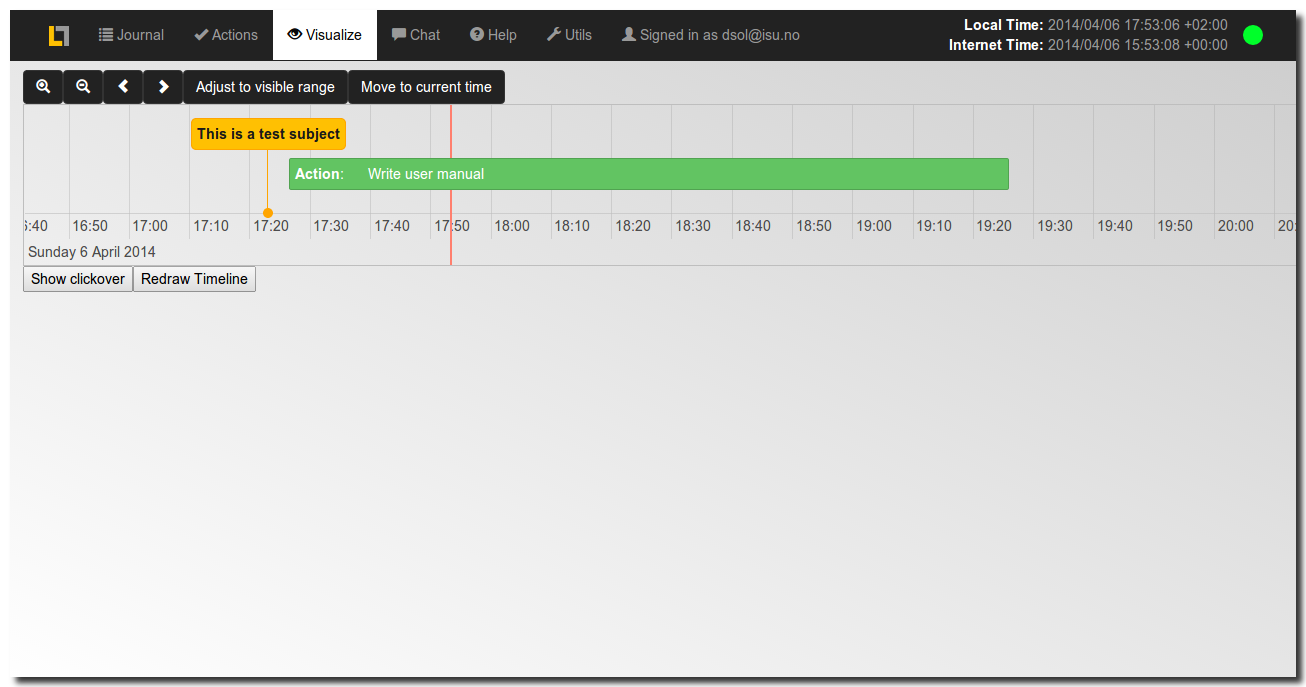
\includegraphics{visualize.png}
\end{figure}

The visualization view is very much under development, and will most likely get an upgrade in the future.


\section{The Chat View}
\label{User manual:the-chat-view}
The chat is very simple in design and features, by which the only feature is to write to all. On the right side you have a list that displays all online users, with a number in parentheses to indicate how much latency they got. i.e. how much time since they were online. If a user have zero in latency, that doesn't need to mean they are online in the chat room, because the latency will update with a frequent interval as long as they have Libellus running.
\begin{figure}[htbp]
\centering

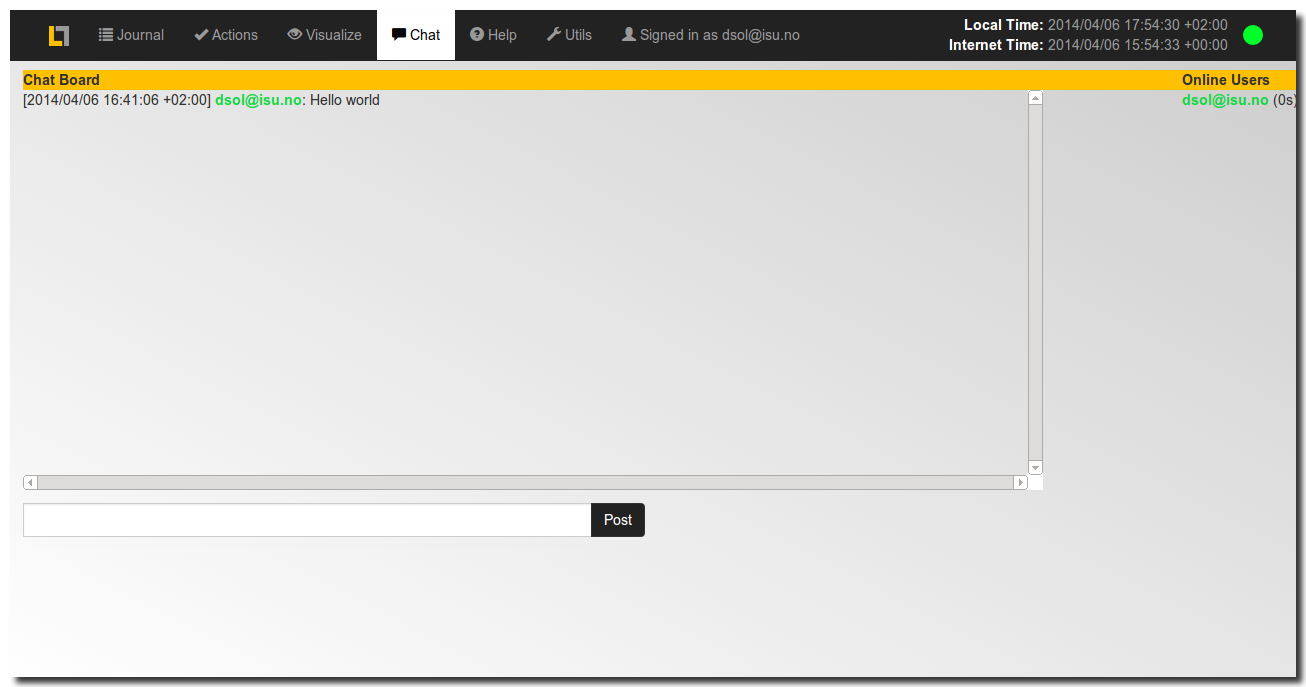
\includegraphics{chat.png}
\end{figure}

The chat is meant to be used for anything that is not important enough to become an independant journal entry, but can really be used to anything. For instance a bulletin board to keep track of who is available or not. Keep in mind that everything you write in the chat will be logged and synchronized with other Libellus instances on the network. The last thing to know is that when you click on the input field, or hit the submit button, you will automaticly be scrolled down to the bottom of the chat history.


\section{The Utils View}
\label{User manual:the-utils-view}
This is a view where you can do multiple tasks, like exporting data and view replication status.
\begin{figure}[htbp]
\centering

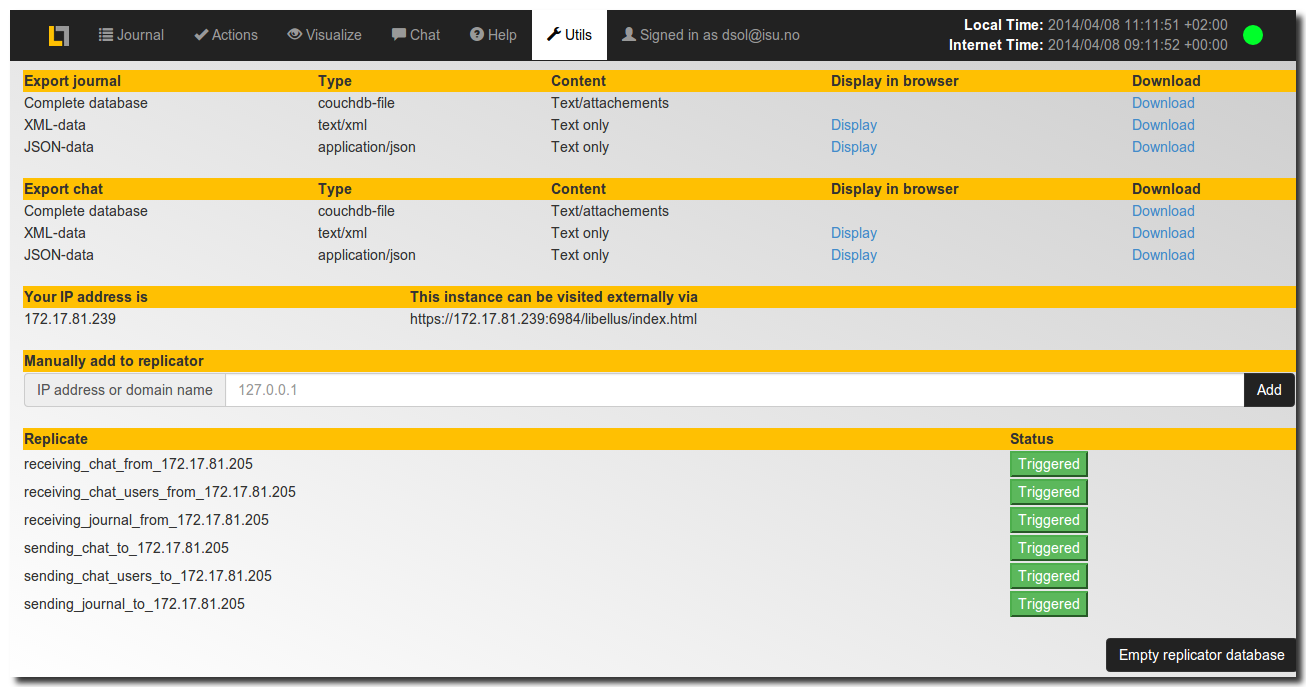
\includegraphics{utils.png}
\end{figure}


\subsection{Export}
\label{User manual:export}
The first section you see is for exporting. Here you can extract the journal and the chat database. You can download the complete and raw database file, which you can save and add back into Libellus later. View the maintenance guide for an explanation for how to do this. If you export as XML or JSON, you don’t get attachments and it’s not possible to import these formats into the database again after exporting. This can be used with import to other software.


\subsection{Visit externally}
\label{User manual:visit-externally}
The section in the middle of the screen is where you can see your own IP address and find the URL for your running instance of Libellus. You can use this to visit your instance externally on other devices, like smartphones or tablets.


\subsection{Add replication}
\label{User manual:add-replication}
At startup Libellus will detect other running instances of the software and add them to the replication automatically. But in some cases it may be useful to manually set up replication to other instance. This can for example be an instance on the Internet which may connect multiple local networks.


\subsection{View status and remove replications}
\label{User manual:view-status-and-remove-replications}
On the bottom you can see the status for all the replications. If the status shows a green box with the caption \emph{Triggered}, like in the image above, everything is as it should. If you see a red box with the word \emph{Error} then something is wrong. This will most likely be the cause of other clients going offline.

Finally you can remove all replications by clicking on the button at the bottom right corner.


\section{Filters}
\label{User manual:filters}
The journal view has filters that can be applied to remove everything you don’t want to see.
There is two possible ways to filter out data, by keyword and datetime. Filtering on both does work, but the last option chosen will be prioritized. The solution is to click on the input field to which you want top priority.


\subsection{Filter by keywords}
\label{User manual:filter-by-keywords}
To search for a word, you can enter it in the input field on the right. All search words will be matched against everything in the journal entry or an appendix related to an entry. You can for example search for a keyword, person, filename or a filed copy. The search is case insensitive and will with each keystroke adjust the filters to create a real time feeling. The button with the trash can, will as implied empty the input field for text.

Here you can see the journal table without any filters. We got two journal entries, which looks almost the same, but with one difference.
\begin{figure}[htbp]
\centering

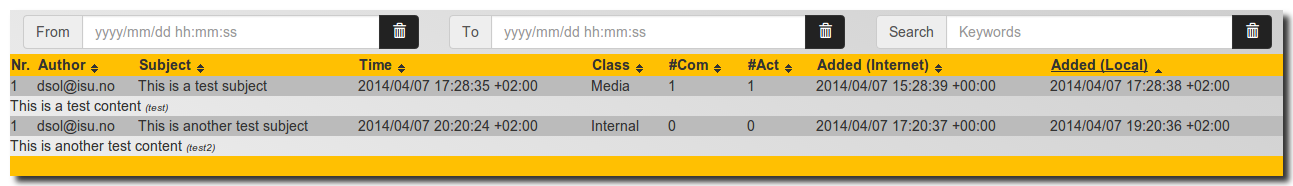
\includegraphics{filter2.png}
\end{figure}

Here is the same table, but here we only show entries that has the word \emph{another} in it.
\begin{figure}[htbp]
\centering

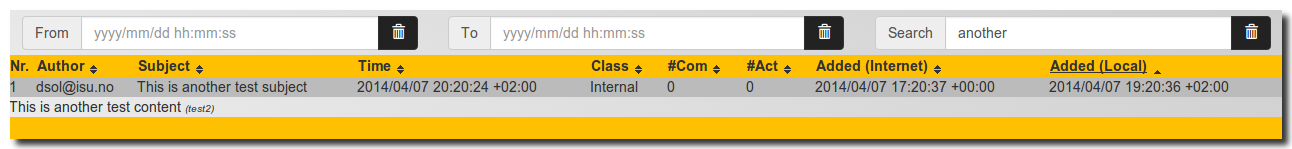
\includegraphics{filter1.png}
\end{figure}


\subsection{Filter by datetime}
\label{User manual:filter-by-datetime}
When filtering on time you have three alternatives. You can use the \emph{From} input field to set a start time, where you will only see entries that has local added time since the date time you choose. This can for instance be used to get all updates after a status meeting.
\begin{figure}[htbp]
\centering

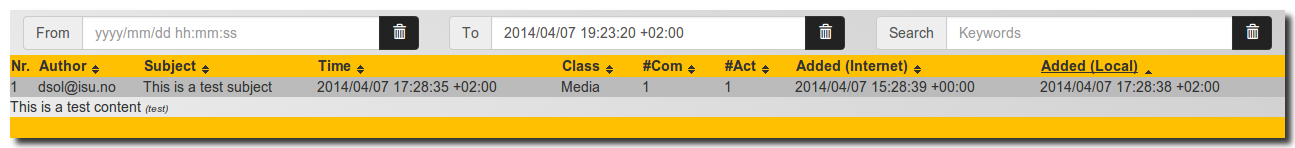
\includegraphics{filter3.png}
\end{figure}

You can also use the \emph{To} option to only show entries up to the given date time.
The last alternative is to use both, to only get entries that is within the time frame from both \emph{To} and \emph{From}.
\begin{figure}[htbp]
\centering

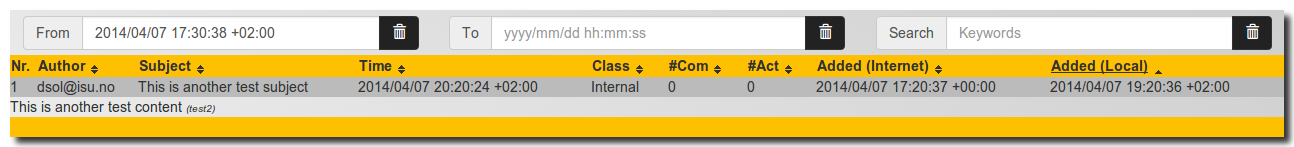
\includegraphics{filter4.png}
\end{figure}


\chapter{3.   FAQ}
\label{FAQ:faq}\label{FAQ::doc}
\textbf{The time sync / offset button is red}

This either means that you don't have Internet connection or that your computer time wrong. If the Internet time displays \emph{N/A}, then you don't Internet access most likely, or that the external source is down. If your computer time is incorrect, then you must change it according to your operating system.

Please verify your Internet connectivity by visiting a external webpage, eg \href{http://www.libellus.no}{http://www.libellus.no}
Then check that nothing is blocking your access to the Internet time server, by opening the following link manually:

\begin{notice}{note}{Note:}
timeapi.herokuapp.com/utc/now.json?callback=jQuery18309364777216687799\_1396946053197\&\_=1396946053268
\end{notice}

If you need to accept a non trusted web page, or are presented with a SSL error, review the sites certificate and see if you can accept it.

\textbf{My local time is in the wrong time zone. How can I change it?}

Open the time and date settings on your operating systems and change it there.

\textbf{How can I sort on several items at the same time?}

Hold down the shift key as you click on the table headers.


\chapter{Changelog}
\label{Changelog::doc}\label{Changelog:changelog}
\textbf{1.0}
\begin{itemize}
\item {} 
Initial release.

\end{itemize}


\chapter{Contributors}
\label{Contributors::doc}\label{Contributors:contributors}



\chapter{Attribution}
\label{Attribution:attribution}\label{Attribution::doc}
The development of this software was made possible using the following components:
\begin{itemize}
\item {} 
CouchDB

\item {} 
Bootstrap

\item {} 
jQuery

\item {} 
Python

\item {} 
sphinx-doc

\item {} 
bootstrapx-clickover.js

\item {} 
bootstrap-dialog.js

\item {} 
jquery.tablesorter.js

\item {} 
jquery.browser.js

\item {} 
jquery.form.js

\item {} 
timeline.js

\item {} 
moment.js

\end{itemize}


\chapter{License}
\label{License::doc}\label{License:license}
\begin{notice}{note}{Note:}
Licensed under the Apache License, Version 2.0 (the ``License''); you may
not use this file except in compliance with the License. You may obtain
a copy of the License at: apache.org/licenses/LICENSE-2.0
\end{notice}



\renewcommand{\indexname}{Index}
\printindex
\end{document}
